\chapter{Постановка задачи распознавания молекулы. Методы решения} \label{ch1}

В данной главе приводится постановка задачи распознавания молекулы. Даются определения основных понятий предметной области и описываются существующие решения.

В параграфе \ref{ch1:sec1} приводится постановка задачи распознавания молекулы. Производится описание входных и выходных данных. В параграфе \ref{ch1:sec2} описана общая структура программ, построенных на  алгоритмах распознавания геометрических примитивов. Такие программы мы будем называть \textbf{rule-based решениями}. В параграфе \ref{ch1:sec3} описаны различные подходы решения задачии распознавания молекулы с использованием методов машинного обучения -- \textbf{ML-based системы}. В параграфе \ref{ch1:sec4} приведён алгоритм сборки молекулы из распознанных тех или иным способом примитивов.

\section{Постановка задачи распознавания молекулы} \label{ch1:sec1}
\subsection{Описание входных данных}
На вход задачи подаётся изображение химической молекулы. В рамках данной задачи конкретизируются следующие требования к изображениям:
\begin{itemize}
	\item Молекула является органической. Это означает, что в молекуле присутствуют только те атомы, которые составляют основу либо присутствуют в органических соединениях: углерод (C), кислород (O), азот (N), водород (H), фосфор (P), фтор (F), кремний (Si), а также хлор (Cl) и бром (Br)
	\item Молекула может быть стереоизомером: на изображении допускаются сплошные и штрихованные клиновидные связи
	\item На изображении отрендерена молекула, являющаяся конкретным изомером, то есть не поддерживаются смеси вида \textit{(R), (S), RS, (RS)}. Также не поддерживаются перечёркнутые связи, обозначающие смесь геометрических (E и Z) изомеров
\end{itemize}

Изображения могут быть получены как из электронных источников литературы, так и из печатных. Допускается наличие дефектов, связанных с небрежным хранением бумажного документа, его возрастом, а также гауссовское зашумление, получаемое в результате процесса сканирования.

Не допускается наличие искажений изображения, получаемых:

\begin{itemize}
	\item при фотографировании на длинной выдержке
	\item при неполном прилегании документа к стеклу сканера
\end{itemize}

\subsection{Описание выходных данных}
Выходные данные представляют из себя стандартизованный текстовый идентификатор InChI \cite{inchi_trust, inchi_wiki}. Данный идентификатор разработан организациями IUPAC и NIST в течение 2000 -- 2005 годов для обеспечения стандартного и читаемого способа кодирования информации о структуре молекулы и облегчить поиск этой информации в различных базах данных. Он позволяет хранить информацию о структурной формуле, стереоизомерии и наличии изотопов.

Важно отметить, что, тем не менее, InChI не всегда способен однозначно закодировать скелетную формулу. Так, при рисовании алленов зачастую вместо одной из двух клиновидных связей рисуют простую одинарную связь, подразумевая при этом клиновидную. Химики так делают, поскольку знают, что молекула со скелетом такого вида может иметь только одну конкретную геометрическую структуру, в связи с чем достаточно нарисовать только один клин. При этом InChI-представления у этих двух скелетных формул будут разными, хотя молекулы являются одинаковыми. Это явление значительно снижает качество распознавания молекул и будет более подробно показано в подразделе \ref{ch1:sec4}.

\section{Rule-based решения} \label{ch1:sec2}
Для подготовки обзора rule-based решений была использована статья \cite{rajan2020review}. В ней описаны 14 различных программных продуктов, реализованных в рамках rule-based подхода. Каждый продукт имеет свои особенности, которые позволяют ему справляться лучше с теми или иными особенностями изображения, однако основной конвейер у них общий и состоит из следующих этапов:
\begin{enumerate}[1.]
	\item \textbf{Предобработка}. Данный этап предполагает бинаризацию изображения, то есть его перевод в оттенки серого, сглаживание изображения --  использование антиалиасинга, фильтров Гаусса и т. п., и утончение линий.
    \item \textbf{Поиск стандартных и клиновидных связей}. Данная операция предполагает обнаружение и классификацию связей. Стандартные связи являются совокупностью от одного до трёх параллельных отрезков, поэтому они могут быть обнаружены с применением детектора Хаффа. Штрихованные клиновидные связи могут быть обнаружены как последовательность увеличивающихся в толщине и ориентированных одинаковым образом равнобедренных трапеций. Сплошные клиновидные связи изображаются как равнобедренный треугольник, основание которого много меньше, чем две его остальные стороны.
    \item \textbf{Поиск ароматических соединений}. Ароматическое соединение -- это циклические углеводороды, обладающие определёнными химическим свойствами, такими как склонность к реакциям замещения. С точки зрения задачи распознавания важно понимать, что ароматическое соединение представляет может быть изображено в виде формулы Кекуле или формулы Полинга -- таким образом, возникает необходимость поиска окружностей внутри циклов и правильного добавления этих соединений в молекулу.
    
    \begin{figure}[ht!] 
    	\center
    	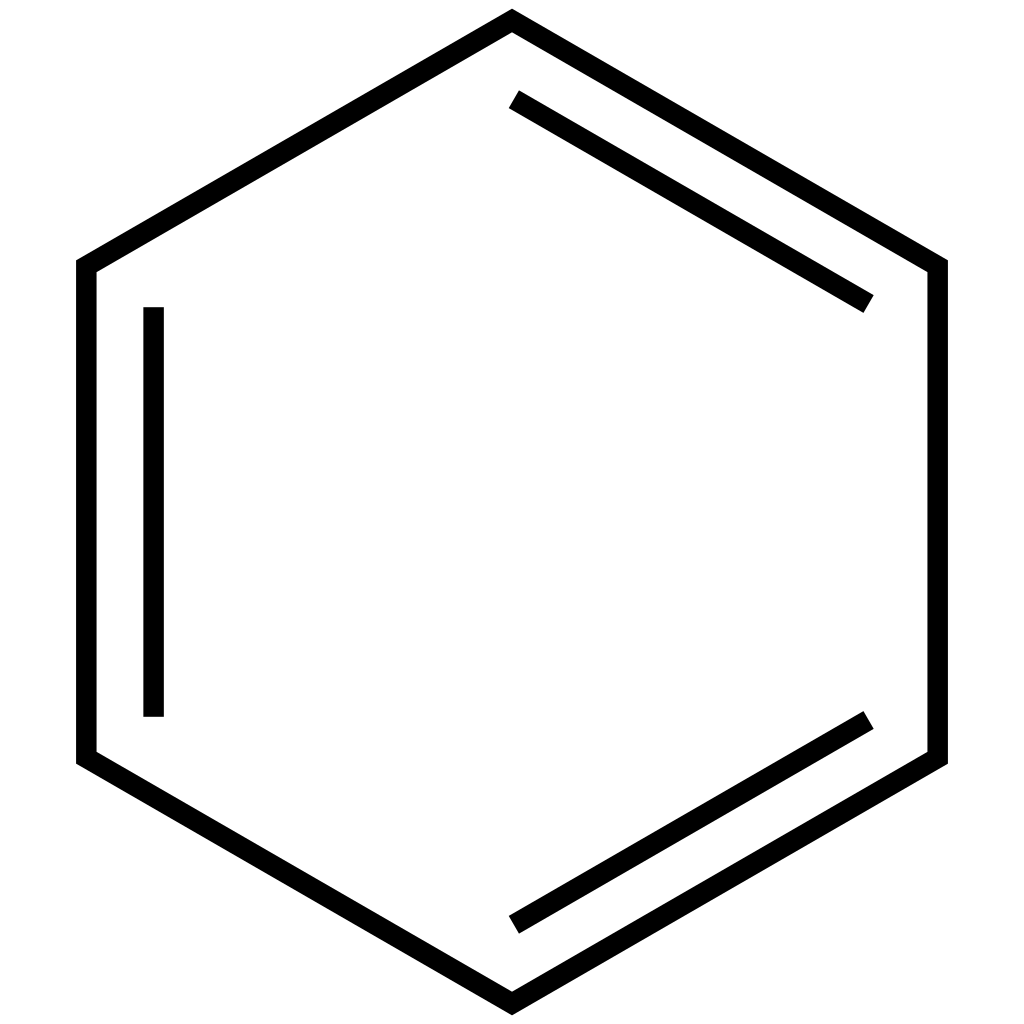
\includegraphics [scale=0.16] {my_folder/images/benzol_kekule}
    	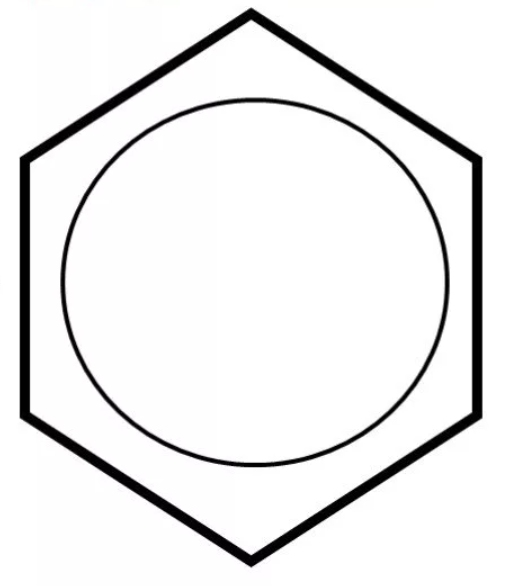
\includegraphics [scale=0.28] {my_folder/images/benzol_poling}
    	\caption{Бензол. (1) Формула Кекуле, (2) Формула Полинга} 
    	\label{fig:benzol}
    \end{figure}
\end{enumerate}

\section{ML-based решения} \label{ch1:sec3}

Согласно \cite{rajan2020review}, до 2019 года было известно два решения, использовавших машинное обучение. Первое из них, OCSR \cite{gkoutos2003chemical}, использовало карты Кохонена для того, чтобы отличать изображения химических молекул от других картинок.Программный продукт ChemOCR использовал машину опроных векторов (\cite{cortes1995support}) для  классификации изображений связей.

Первый продукт, полностью построенный на технологиях машинного обучения, называется MSE-DUDL и представлен в 2019 году \cite{staker2019molecular}. Ивзестно, что в основе этого продукта лежит свёрточная сеть на базе U-Net. Модель была натренирована на 57 миллионах изображений, сгенерированных пакетом Indigo.

Второй продукт, Chemgrapher, содержит две сети. Одна отвечает за обнаружение объектов, а вторая -- за их классификацию. Обе сети являются свёрточными, и были натренированы на изображениях, сгенерированных пакетом RDKit. В результате исследований этого решения было выяснено, что сегментирующая нейронная сеть имеет гораздо более низкое качество, чем классифицирующая.

\section{Решение на базе нейросети-трансформера}

Стоит отдельно упомянуть решения, построенные на нейросетях с архитектурой <<трансформер>>.

Отличием трансформера от классических CNN и RNN является наличие механизма внимания Multi-Head Attention.

Данная архитектура сетей чаще всего применяется при решении задачи машинного перевода, поэтому описывать принцип её работы мы здесь будем в терминах текстов. Тем не менее, как и любая нейронная сеть, трансформер может принимать на вход любые конечные последовательности данных, в частности изображения молекул.

\begin{figure}[ht!] 
	\center
	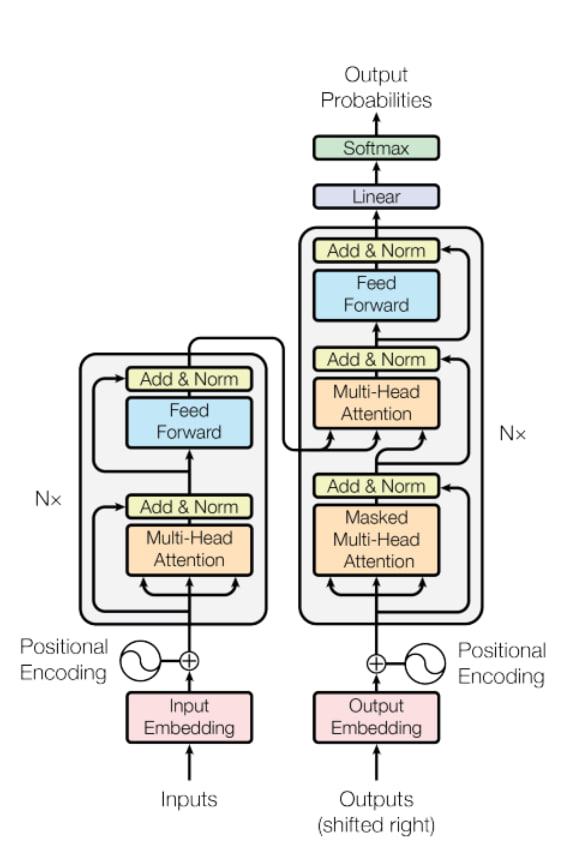
\includegraphics [scale=0.6] {my_folder/images/transformer}
	\caption{Архитектура сети <<трансформер>>} 
	\label{fig:transformer}
\end{figure}

В данной архитектуре все слова параллельно проходят через заданные слои. На пути каждого слова находится слой внимания, суть которого заключается в возможности взаимодействия с другими словами.

На вход слою внимания даются вектора Query и несколько пар Key и Value.  Чаще всего при практическом использовании оказывается, что  Key и Value это один и тот же вектор. Каждый из них преобразуется обучаемым линейным преобразованием, а потом вычисляется скалярное произведение Q со всеми K по очереди, результат этих скалярных произведений подаётся на вход в softmax слой, и с полученными весами все вектора V суммируются в единый вектор. 

\begin{figure}[ht!] 
	\center
	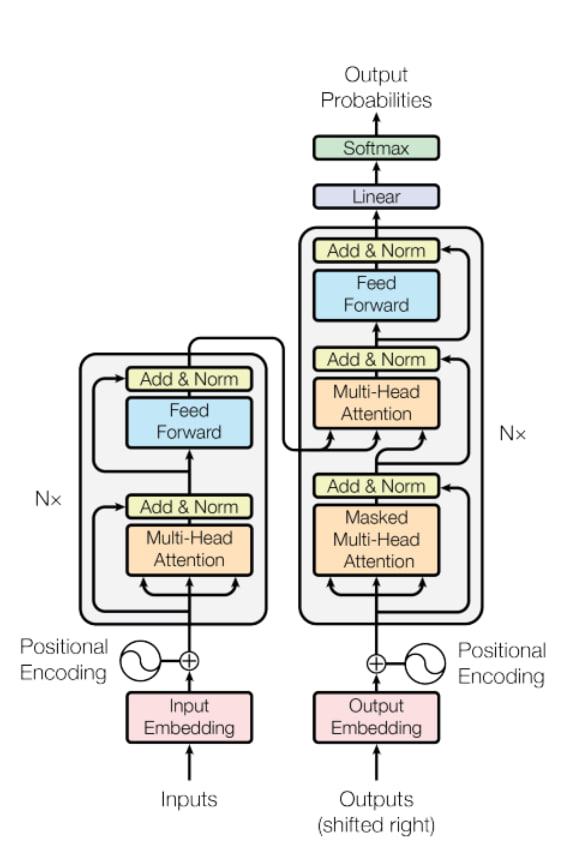
\includegraphics [scale=0.6] {my_folder/images/transformer}
	\caption{Архитектура слоя внимания} 
	\label{fig:attention}
\end{figure}

Данный подход позволяет обучать сеть искать похожие в каком-то смысле слова и таким образом <<уделять внимание>> наиболее значимым словами при произведении машинного перевода. 

Несмотря на то, что трансформеры изначально задумывались как нейросети для машинного перевода, они нашли также применение в других задачах. Например, можно обучить трансформер таким образом, чтобы он на вход получал изображение, а на выход отдавал текстовую последовательность.
Одним из примеров таких сетей является сеть DETR от FacebookResearch \cite{detr}.

На базе трансформера в рамках kaggle-соревнования BMS \cite{bms} было разработано решение, которое конвертирует изображение молекулы \textit{целиком} в InChI-последовательность. Оказалось, что трансформер решает задачу распознавания структуры молекулы даже лучше, чем object-detection модель, из чего можно сделать вывод, что механизм внимания позволяет сети обучаться искать взаимосвязь между скелетной формулой и InChI-цепочками. Данное наблюдение ещё раз показвыает способность трансформеров к обучению языкам, поскольку InChI-последовательность, как и скелетная формаула, является языком описания структуры молекулы.


\section{Алгоритм сборки молекулы} \label{ch1:sec4}
При решении задачи распознавания молекулы любым из описанных выше способов возникает необходимость собрать молекулу из отдельных примитивов. Приведём здесь алгоритм, который позволяет это делать.

На вход алгоритма подаётся набор изображений связей и меток атомов. Будем строить \textit{граф молекулы} -- граф, в вершинах которого находятся атомы (непомеченные атомы углерода либо другие атомы с указанием названия), а рёбрами которого являются связи.

Такой граф можно передать в один из химических пакетов. В рамках данной работы используется Python-реализация пакета RDKit. Данный пакет позволяет:
\begin{itemize}
	\item Строить граф молекулы из таких распространённых форматов, как SMILES, SDF, InChI
	\item Добавлять атомы и связи в существующий граф молекулы, а также указывать категорию связи
	\item Генерировать текстовые идентификаторы SMILES, SDF, InChI из графа молекулы
\end{itemize}

Таким образом, для генерации InChI-идентификатора достаточно правильным образом сформировать граф молекулы.

Будем считать, что связи представлены в баундбоксов, для которых указана категория связи и её направление. В случае плоской связи достаточно указать направление диагонали, в случае стереосвязи -- её начало и конец. Метки атомов также ожидаются в виде баундобксов, для которых указан текст метки.

Граф строится в несколько этапов.

Первый этап -- построение списка смежности молекулы. Для этого производится двойное вложенное итерирование по списку связей и, если у бсвязей находится общая точка (пересечение баундбоксов с учётом направления связи внутри баундбокса), то точка соединения объявляется новым атомом. Если атом уже существует в списке смежности, то текущая связь добавляется в него. Иначе, создаётся новый элемент в списке смежности и к нему присоединяется две связи.

Второй этап -- поиск висячих вершин, то есть непомеченных атомов, которые связаны только с одним другим атомом.

Третий этап -- сопоставление помеченных и непомеченных атомов. Для этого производится итерирование по всем возможным парам вершин графа молекулы и меток атомов и, если метка расположена достаточно близко к вершине, то считается, что метка относится к данной вершине.

Последний этап -- добавление построенного списка смежности в rdkit-молекулу. После того, как атомы и связи добавлены, необходимо вызвать генератор центров хиральности. Он позволяет сгенерировать данные, необходимые для вывода InChI-идентификатор из информации о клиновидных связях. Важно заметить, что RDKit самостоятельно выводит количество присоединённых атомов водорода из того набора связей, который текущий атом имеет со своими соседями. Это обстоятельство позволяет при классификации меток атомов опеределять в одну категорию метки с явным указанием присоединённых атомов водорода и без него.

Неприятным моментом является тот факт, что на данном этапе происходят основные потери точности сборки, связанные с неоднозначным соответствием строения химической молекулы и необходимым набором клиновидных связей, о котором упоминалось во введении.

%
%\begin{table} [htbp]% Пример оформления таблицы
%	\centering\small
%	\caption{Представление данных для сквозного примера по ВКР \cite{Peskov2004}}%
%	\label{tab:ToyCompare}		
%		\begin{tabular}{|l|l|l|l|l|l|}
%			\hline
%			$G$&$m_1$&$m_2$&$m_3$&$m_4$&$K$\\
%			\hline
%			$g_1$&0&1&1&0&1\\ \hline
%			$g_2$&1&2&0&1&1\\ \hline
%			$g_3$&0&1&0&1&1\\ \hline
%			$g_4$&1&2&1&0&2\\ \hline
%			$g_5$&1&1&0&1&2\\ \hline
%			$g_6$&1&1&1&2&2\\ \hline		
%		\end{tabular}	
%	\normalsize% возвращаем шрифт к нормальному
%\end{table}


% \firef{} от figure reference
% \taref{} от table reference
% \eqref{} от equation reference


%Формулы могут быть размещены в несколько строк. Чтобы выставить номер формулы напротив средней строки, используйте окружение \verb|multlined| из пакета \verb|mathtools| следующим образом \cite{Ganter1999}:
%
%\begin{equation} 
%\label{eq:fConcept-order-ch1}
%\begin{multlined}
%(A_1,B_1)\leq (A_2,B_2)\; \Leftrightarrow \\  \Leftrightarrow\; A_1\subseteq A_2\; \Leftrightarrow \\ \Leftrightarrow\; B_2\subseteq B_1. 
%\end{multlined}
%\end{equation}


%Используя команду \verb|\labelcref| из пакета \verb|cleveref|, допустимо следующим образом оформлять ссылку на несколько формул:
%(\labelcref{eq:Pi-ch1,eq:fConcept-order-ch1}).
%
%
%\input{my_folder/tex/fig-spbpu-whitehall-three-in-one} % пример подключения 3х иллюстрации в одном рисунке

%Пример ссылок \cite{Article,Book,Booklet,Conference,Inbook,Incollection,Manual,Mastersthesis,Misc,Phdthesis,Proceedings,Techreport,Unpublished,badiou:briefings}, а также ссылок с указанием страниц, на котором отображены номера страниц  \cite[с.~96]{Naidenova2017} или в виде мультицитаты на несколько источников \cites[с.~96]{Naidenova2017}[с.~46]{Ganter1999}. Часть библиографических записей носит иллюстративный характер и не имеет отношения к реальной литературе. 



%\FloatBarrier % заставить рисунки и другие подвижные (float) элементы остановиться

%% Вспомогательные команды - Additional commands
%
%\newpage % принудительное начало с новой страницы, использовать только в конце раздела
%\clearpage % осуществляется пакетом <<placeins>> в пределах секций
%\newpage\leavevmode\thispagestyle{empty}\newpage % 100 % начало новой страницы